% !!!!!!!!!!!!!!!!!!   ВНИМАНИЕ !!!!!!!!!!!!!!!!!!!!!!!!!!!!!!!!!!!!!!!!!!!!!!!!!!!!!!!!!
% Заголовки разделов формируются при помощи команд \section{}, \subsection{}, \subsubsection{}
% Не используйте уровень вложенности заголовков больше трех!
% -----------------------------
% Для оформления теорем, лемм, следствий используйте окружения 
% Def     - Определение
% Teor    - Теорема
% Lem     - Лемма
% Predl   - Предложение
% Ass     - Утверждение
% Cor     - Следствие
% Example - Пример
% -----------------------------
% Доказательство теоремы начинается командой \proof и завершается командой \endproof
% -----------------------------
% Литература помещается в окружение biblio.

\documentclass[11pt, oneside, a4paper]{article}
%\usepackage[cp1251]{inputenc} % кодировка
\usepackage[utf8]{inputenc} % кодировка
\usepackage[english, russian]{babel} % Русские и английские переносы
\usepackage{graphicx}          % для включения графических изображений
\usepackage{cite}              % для корректного оформления литературы
\usepackage{enumitem}
\usepackage{amsmath,amsthm,amssymb}
\usepackage{mathtext}
\usepackage{array}
\usepackage{hyperref}


%стилевой пакет
\usepackage{schoolseminar2022}


\begin{document}
% \udk     - универсальный десятичный классификатор
% \msc     -
% \title   - название статьи
% \authors - список авторов

\setcounter{page}{1}

\udk{519.853.4, 004.032.26}

\title{Использование аппроксимации нейронными сетями при решении задач глобальной оптимизации\footnote{Работа выполнена при поддержке Министерства науки и высшего образования РФ (проект \textnumero~0729-2020-0055) и научно-образовательного математического центра <<Математика технологий будущего>> (проект \textnumero~075-02-2021-1394).}}


\authors{Карпенко С.Н., Лебедев И.Г., Надумин Д.В.}
\organizations{ННГУ им. Н.И. Лобачевского\\
Институт информационных технологий, математики и механики}



\abstractru{
В работе рассматривается задача поиска глобального минимума многоэкстремальной функции. Для решения этой задачи был выбран алгоритм имитации отжига. Для ускорения процесса поиска минимума используется аппроксимация целевой функции нейросетью. Представлены результаты работы комбинированного алгоритма глобальной оптимизации, объединяющего алгоритм имитации отжига, использующего нейронную сеть для аппроксимации функций и метод Нелдера-Мида для точного решения задачи оптимизации.  В данной работе проводились эксперименты с серией двумерных функций из генератора GKLS. Результаты показывают сокращение числа вычислений целевой функции при сохранении высокой точности поиска.
}

\keywords{методы оптимизации, глобальная оптимизация, нейронные сети, машинное обучение.}


% \section{название} - заголовок раздела первого уровня
% \subsection{название} - заголовок раздела второго уровня
% \subsubsection{название} - заголовок раздела третьего уровня
% Не используйте уровень вложенности заголовков больше трех!
% Каждый абзац текста в статье начинается командой \par или пустой
% строкой.

\bigskip

\section{Введение}

Нейронная сеть представляет собой математическую модель, построенную по принципу организации и функционирования биологических нейронных сетей – сетей нервных клеток живого организма. Это понятие возникло при изучении процессов, протекающих в мозге, и при попытке смоделировать эти процессы. 

С точки зрения математики, обучение нейронных сетей - это многопараметрическая задача нелинейной оптимизации. С точки зрения развития вычислительной техники и программирования, нейронная сеть - способ решения проблемы эффективного параллелизма.

Нейронные сети применяются для решения многих прикладных задач. Наиболее известными сферами применений нейронных сетей являются: распознавание образов и классификация, прогнозирование, аппроксимация.
Нейронные сети могут аппроксимировать непрерывные функции. С помощью линейных операций и каскадного соединения можно из произвольного нелинейного элемента получить устройство, вычисляющее любую непрерывную функцию с некоторой наперёд заданной точностью.

История нейронных сетей намного длиннее, чем принято считать. Сама идея "способной к мышлению системы" возникла еще в Древней Греции, и популярность нейронных сетей менялась с течением времени. 

В 1943 году Уоррен Маккалок и Уолтер Питтс опубликовали работу «Логическое исчисление идей, относящихся к нервной деятельности» \cite{fio_bib3}. Целью данного исследования было изучение работы человеческого мозга. В 1958 году, Фрэнк Розенблатт в своем исследовании «Персептрон: вероятностная модель хранения и организации информации в головном мозге» \cite{fio_bib4} описал модель персептрона. В 1974 году, первым ученым на территории США, описавшим в своей диссертации \cite{fio_bib5} использование алгоритма обратного распространения ошибки в нейронных сетях, стал Пол Вербос, хотя развитием этой идеи занимались многие исследователи. В 1989 году, Янн Лекун опубликовал статью \cite{fio_bib6}, в которой было описано практическое использование ограничений обратного распространения ошибки и интеграция в архитектуру нейронной сети для обучения алгоритмов. 

\section{Постановка задачи глобальной оптимизации}
Задача многомерной многоэкстремальной оптимизации может быть определена как проблема поиска наименьшего значения действительной функции $\phi(y)$

\begin{equation*}   %%%%%%%%
\phi(y^*) = min\{\phi(y):y\in D\},
\end{equation*}
\begin{equation}   %%%%%%%%
D = \{y \in R^N : a_i \leq y_i \leq b_i,
1 \leq i \leq N \},
\end{equation}
где $a,b \in R$ - заданные векторы.


Численное решение задачи (1) к построению оценки $y_k^* \in D$, отвечающей некоторому понятию близости к точке $y^*$ (например, $\parallel y^*-y_k^* \parallel \leq \epsilon$, где $\epsilon>0$ это некоторая заданная точность) на основе конечного числа $k$ вычислений оптимизируемой функции. Относительно класса рассматриваемых задач предполагается выполнение двух важных условий:
\begin{enumerate}
\item Предполагается, что оптимизируемая функция $\phi(y)$ может быть задана алгоритмически, как результат работы некоторой подпрограммы или библиотеки.

\item Будем предполагать, что $\phi(y)$ удовлетворяет условию Липшица
\begin{equation}
|\phi(y_1)-\phi(y_2)|\leq L\parallel y_1-y_2 \parallel
,y_1,y_2 \in D, 0<L< \infty
\end{equation}
\end{enumerate}
что соответствует ограниченности изменения значений функции при ограниченной вариации аргумента. Это предположение можно интерпретировать (применительно к прикладным задачам) как отражение ограниченности мощностей, порождающих изменения в моделируемой системе.

Задачи многоэкстремальной оптимизации имеют существенно более высокую трудоемкость решения по сравнению с другими типами оптимизационных задач, т.к. глобальный оптимум является интегральной характеристикой решаемой задачи и требует исследования всей области поиска. Как результат, поиск глобального оптимума сводится к построению некоторого покрытия (сетки) в области параметров, и выборе наилучшего значения функции на данной сетке. Вычислительные затраты на решение задачи растут экспоненциально с ростом размерности \cite{fio_bib7}.


\section{Метод имитации отжига}
Алгоритм имитации отжига является общим алгоритмическим методом решения задачи глобальной оптимизации. Он основывается на имитации физического процесса, который происходит при кристаллизации вещества, в том числе при отжиге металлов.

При помощи моделирования такого процесса ищется такая точка или множество точек, на котором достигается минимум некоторой числовой функции $\phi(y^i),y^i=(y_1,...y_n)\in Y$. Решение ищется последовательным вычислением точек пространства $Y$\cite{fio_bib16}, \cite{fio_bib20}. 


Введём следующие обозначения: $Y$ - множество всех состояний системы, $y_i$-состояние на $i$-ом шаге алгоритма; $t_i$-температура на $i$-ом шаге.


Определим три функции:
\begin{enumerate}
\item Функция энергии(то, что оптимизируем):   $E:Y\rightarrow R$
\item Функция изменения температуры с течением времени:  
$T:N\rightarrow R$
\item Функция, порождающая новое состояние:  
$\phi:Y\rightarrow Y$
\end{enumerate}
На входе минимальная $t_{min} $ и начальная $t_{max}$ температуры. Задаём произвольное первое состояние $y_1$ и $t_{min}=t_{max}$.

Пока $t_i>t_{min}$:
\begin{enumerate}
\item $y_c=\phi(y_{i-1})$,
\item $\triangle E=E(y_c)-E(y_{i-1})$,
\item Если $\triangle E \leq 0$, то $y_i=y_c$. Если $\triangle E >0$, то переход осуществляется с вероятностью $P(\triangle E)=e^{- \triangle E /t_i}$,
\item Понижаем температуру $t_{i+1}=T(i)$.
\end{enumerate}
Возвращаем последнее состояние $y$. 

Преимуществом метода имитации отжига является возможность избежать локальные минимумы оптимизируемой функции за счет принятия изменений, временно ухудшающих результат, что отражает суть процесса нагрева расплава для предотвращения его быстрого остывания. Еще одним преимущество – даже в условиях нехватки вычислительных ресурсов для нахождения глобального минимума метод отжига выдает один из локальных минимумов. 

\section{Метод Нелдера-Мида}
Метод Нелдера-Мида является методом безусловной оптимизации \cite{fio_bib19} функции нескольких  переменных $\phi(y^1,...,y^n )$, не использующий градиентов функции. Он относится к группе методов прямого поиска, так как в нем не используются производные. Метод является развитием симплексного метода.
 
Идея метода заключается в следующем: в пространстве $R^N$ выбираются $(n+1)$ пробных векторов, в каждом из которых можно вычислить значение целевой функции. Вершина с наихудшим значение целевой функции -- $A$ отражается через центр тяжести других вершин многогранника, в результате чего из оставшихся вершин строится новый многогранник, называемый отраженным, и одна точка, расположенная на линии проекции на соответствующем расстоянии от центра тяжести.

Метод находит локальный экстремум и может "застрять" в одном из них. Предполагается что функция определена во всех точках области определения.

\section{Математический аппарат нейронной сети прямого распространения}
Согласно универсальной теореме аппроксимации (теореме Цыбенко), доказанной Джорджем Цыбенко в 1989 году, искусственная нейронная сеть с прямым распространением может аппроксимировать любую непрерывную функцию многих переменных с любой точностью. Условиями являются: достаточное количество нейронов скрытого слоя, удачный подбор весов и смещений.

На входе нейронная сеть принимает набор значений переменной. Далее эти значения умножаются на некоторые весовые коэффициенты. После чего в качестве взвешенной по весовым коэффициентам суммы подаются  на вход  каждого из нейронов скрытого слоя, где к этой сумме прибавляется смещение (bias). В результате получаем число, которое подаётся на вход активационной функции. Результат активационной функции и есть выходные значение одного нейрона.

Взвешенная сумма представлена ниже:
\begin{equation}
z = \sum_{i=1}^n y_i \cdot w_i +bias,
\end{equation}
где $bias$ – смещение, $w_i$ – весовой коэффициент, $y_i$ - входное значение.

Далее (3) подаётся в качестве входного значения в активационную функцию. Существует несколько видов активационных функций. В данной работе применялась сигмоидальная функции, область значений которой от 0 до 1.
\begin{equation}
\sigma(z)= \frac{1}{1+e^{-z}}
\end{equation}

\section{Комбинированный алгоритм глобальной оптимизации}
Нами разработан комбинированный алгоритм глобальной оптимизации, использующий нейронную сеть для аппроксимации функций, метод имитации отжига для поиска глобального оптимума и метод Нелдера-Мида для уточнения найденного решения. 

В данной работе была выбрана нейронная сеть прямого распространения (feedforward neural network)\cite{fio_bib2,fio_bib3,fio_bib4,fio_bib5,fio_bib6,fio_bib7} из библиотеки Keras\cite{fio_bib15}. 

В ходе исследования параметры нейронной сети были подобраны следующим образом: 5 слоёв по 32 нейрона в каждом слое. В качестве активационной функции выбрана сигмоида. Весовые коэффициенты имеют нормальное распределение со средним равным 0 и стандартным отклонением равным 0,2, что позволяет задавать их значения от -1 до 1. Смещение нейрона (bias) инициализируется 0. В выходном слое только один нейрон. 

Сам комбинированный алгоритм можно разбить на три пункта:
\begin{enumerate}
\item Создание обучающей выборки для нейронной сети.
\item Обучение нейронной сети.
\item Пока не выполнен критерий остановки, либо пока не выполнено ограничение на количество вычислений целевой функции делаем следующее:
\begin{enumerate}
\item Оптимизация нейросетевой аппроксимации с помощью алгоритма имитации отжига.
\item Оптимизация целевой функции с помощью локального метода, где в качестве первоначального значения используется найденная глобальным методом точка.
\item Если разница между найденным значением и глобальным минимумом меньше 0,01, то комбинированный алгоритм сошёлся.
\item Иначе добавляем в обучающую выборку 10 случайных точек и найденную локальным методом точку.
\item После чего, заново обучаем нейронную сеть и уходим на следующую итерации.
\end{enumerate}
\end{enumerate}
\section{Описание программной реализации}
Программная реализация выполнена на языке Python с помощью библиотек Numpy \cite{fio_bib12}, Matplotlib \cite{fio_bib13}, SciPy \cite{fio_bib14}, Keras \cite{fio_bib15}. 	

Работа выполнялась в среде Jupyter Notebook. Программа разбита на 5 блоков:
\begin{enumerate}
\item Импортируются все библиотеки, в том числе пользовательские функции (в частности, функция нормализации значений) и генератор задач GKLS. 
\item Определена функция задания нейросети, принимающая в качестве аргумента размерность задачи. Функция возвращает объект нейронной сети.
\item Задаётся обучающая выборка, состоящая из 225 значений в области определения функций генератора GKLS.
\item Задаются параметры нейросети и критерии остановки комбинированного алгоритма. Количество эпох обучения равно 6000. Размер выборки для обучения (batch size) на каждой эпохе (каждой итерации) равен одной трети от всего размера обучающей выборки.
\item Выполнение комбинированного алгоритма. В случае повторения обучения нейросети batch size также задаётся равным одной трети от всей выборки с учётом добавленных точек.
\end{enumerate}

\section{Эксперименты}
Эксперименты проводились на компьютере со следующими характеристиками:
\begin{enumerate}
\item Процессор Intel Core i3-9100F, 4100 MHz.
\item ОЗУ 16 Gb (2x8 Gb) DDR4.
\item Видеокарта GeForce GTX 1050 2 Gb.
\end{enumerate}

Задача экспериментов состояла в том, чтобы уменьшить количество вычислений целевой функции. 

На рис.1 представлена поверхность одной из функции генератора GKLS, на рис.2 - её аппроксимация нейросетью.
\begin{figure}[!h]
	\begin{center}
		\begin{minipage}[h]{0.45\linewidth}
			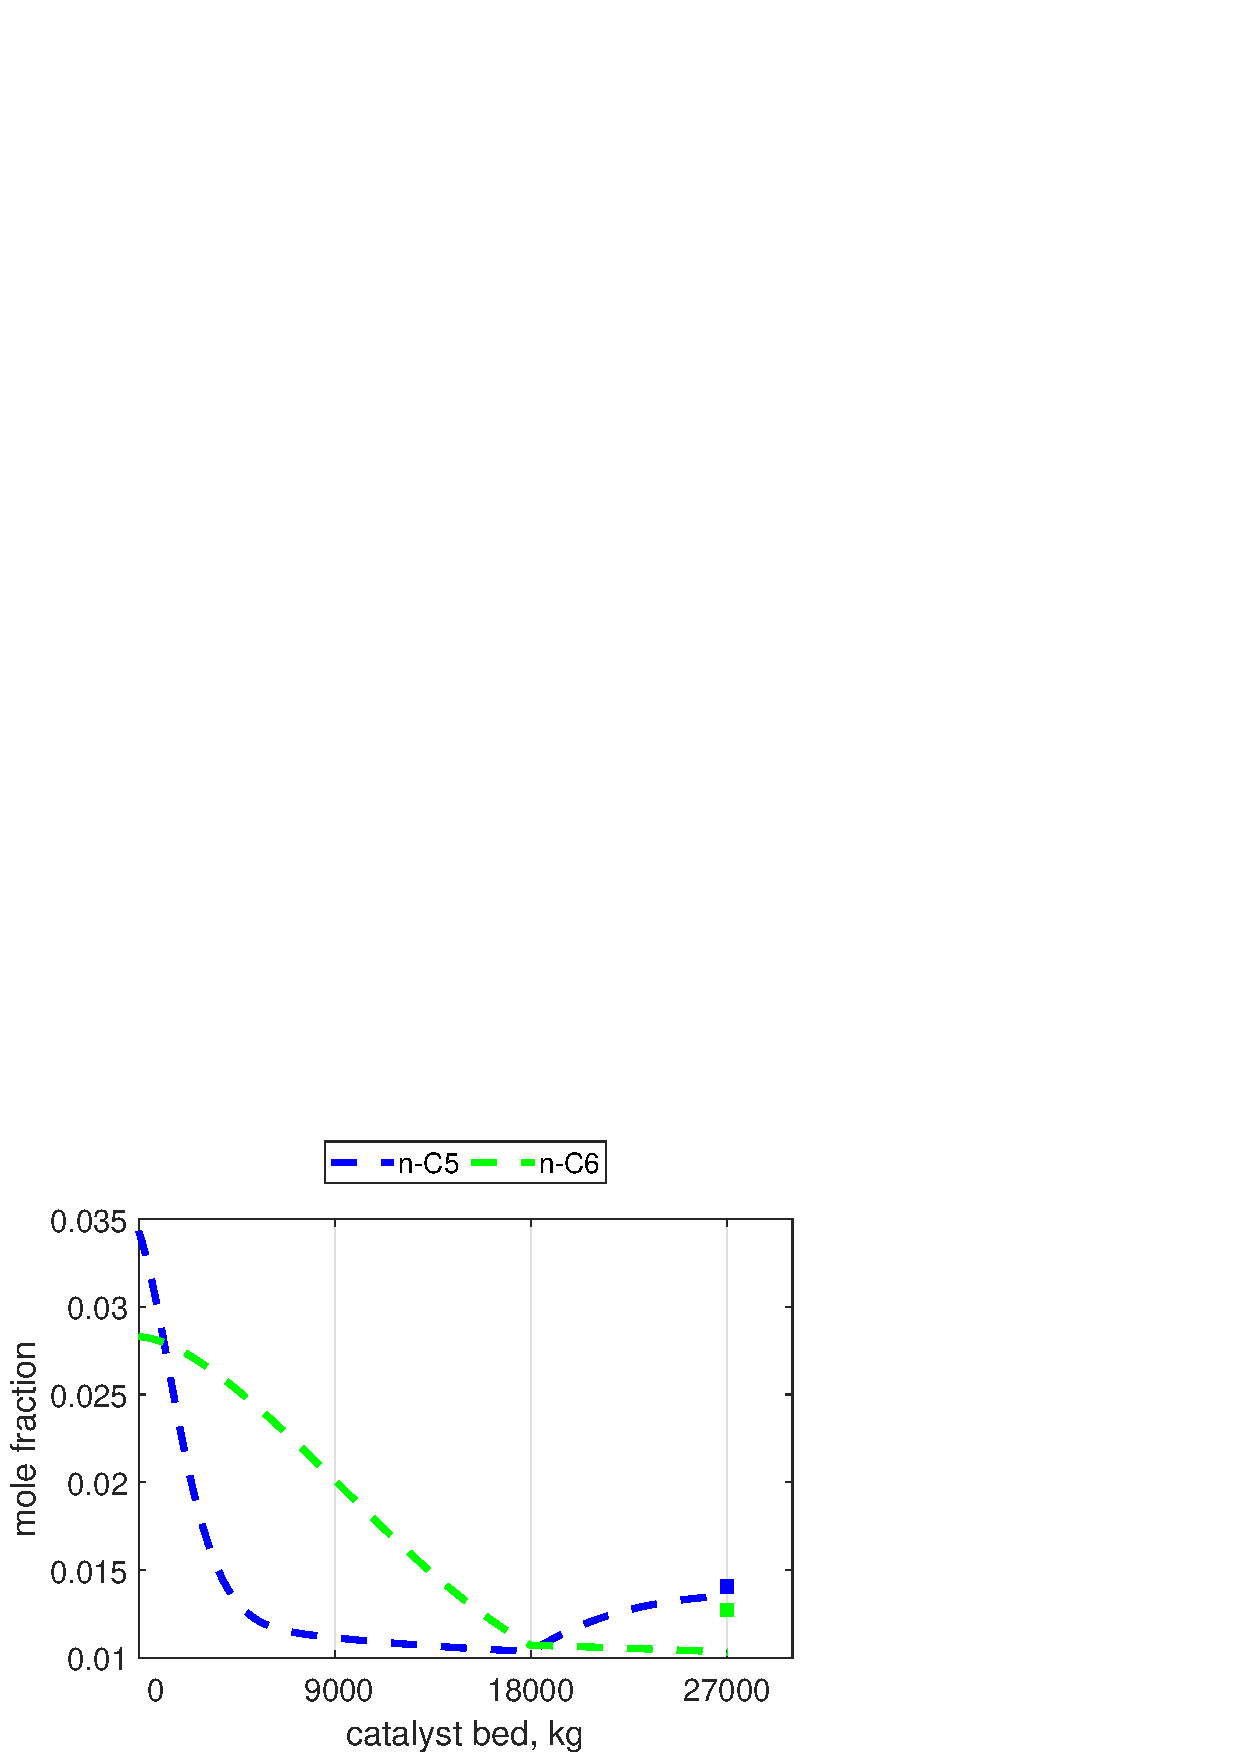
\includegraphics[width=1\linewidth]{figure/1.png}
			\caption{Поверхность функции.} %% подпись к рисунку
		\end{minipage}
		\hfill
		\begin{minipage}[!h]{0.45\linewidth}
			\includegraphics[width=1\linewidth]{figure/1_approx.png}
			\caption{Аппроксимация.}
		\end{minipage}
	\end{center}
\end{figure}	

\newpage



Эксперименты проводились на 10-ти двумерных задачах из генератора GKLS. В работе \cite{fio_bib19} \cite{fio_bib20} описан GKLS-генератор, позволяющий порождать задачи многоэкстремальной оптимизации с заранее известными свойствами: количеством локальных минимумов, размерами их областей притяжения, точкой глобального минимума, значением функции в ней и т.п. 

В таблице 1 отражено среднее число вычислений целевой функции, которые выполнили метод имитации отжига и разработанный нами комбинированный алгоритм, при решении серии задач. Также приведена средняя точность нахождения решения. Максимальное число итераций алгоритма имитации отжига составляло $10000$, остальные параметры соответствуют значениям по умолчанию. 

\begin{table}
	\caption{Результаты работы имитации отжига и комбинированного алгоритма}
	\begin{center}
		\begin{tabular}{|m{3.8cm}|m{6cm} |m{6cm}|}
			\hline
			 & Среднее количество вычислений целевой функции & Точность нахождения решений\\
			 \hline
			 Имитация отжига & 4255,9 & $1,8 \cdot 10^{-8}$\\
			 \hline 
			 Комбинированный алгоритм & 293,4 & $3,3 \cdot 10^{-5}$\\
			 \hline
		\end{tabular}
	\end{center}
\end{table}

Результаты экспериментов показывают значительное уменьшение количества вычислений целевой функции. При этом сохраняется высокая точность нахождения минимума.


\begin{biblio}

\bibitem{fio_bib2}
Cybenko, G. V. Approximation by Superpositions of a Sigmoidal function. Mathematics of Control Signals and Systems. — 1989. — Т. 2, № 4. — С. 303—314.

\bibitem{fio_bib3}
Warren S. McCulloch, Walter Pitts // California State University. – Режим доступа: \url{https://home.csulb.edu/~cwallis/382/readings/482/mccolloch.logical.calculus.ideas.1943.pdf}

\bibitem{fio_bib4}
F. Rosenblatt // Cornell Aeronautical Laboratory. – Режим доступа: \url{https://citeseerx.ist.psu.edu/viewdoc/download?doi=10.1.1.335.3398&rep=rep1type=pdf}

\bibitem{fio_bib5}
Paul Werbos // National Science Foundation. – Режим доступа: \url{https://www.researchgate.net/publication/35657389_Beyond_regression_new_tools_for_prediction_and_analysis_in_the_behavioral_sciences}

\bibitem{fio_bib6}
Y. LeCun, B. Boser // AT \& T  Bell Laboratories. – Режим доступа: \url{http://yann.lecun.com/exdb/publis/pdf/lecun-89e.pdf}

\bibitem{fio_bib7}
Гермейер Ю.Б. Введение в теорию исследования операций / Гермейер Ю.Б. – М.: «Наука», 1971. – 384 c.

\bibitem{fio_bib12}
Официальный сайт библиотеки NumPy. – Режим доступа: \url{https://numpy.org/}

\bibitem{fio_bib13}
Официальный сайт библиотеки Matplotlib. – Режим доступа: \url{https://matplotlib.org/}

\bibitem{fio_bib14}
Официальный сайт библиотеки SciPy. – Режим доступа: \url{https://scipy.org/}

\bibitem{fio_bib15}
Официальный сайт библиотеки Keras. – Режим доступа: \url{https://keras.io/}

\bibitem{fio_bib16}
Kirkpatrick, S.; Gelatt Jr,C.D.;Vecchi, M. P. (1983). "Optimization by Simulated Annealing". Science. 220 (4598): 671–680.

\bibitem{fio_bib19}
Gaviano, M. Software for generation of classes of test functions with known local and global minima for global optimization/ M. Gaviano, D. Lera, D. E. Kvasov, Y. D. Sergeyev // ACM Transactions on Mathematical Software. – 2003. – Vol.  29. – P. 469-480.

\bibitem{fio_bib20}
Сергеев, Я.Д. Диагональные методы глобальной оптимизации / Я.Д. Сергеев, Д.Е. Квасов – М.: Физматлит, 2008. – 352 c.

\end{biblio}


\newpage

\msc{90C26, 82C32}

\title{The using neural network approximation in global optimization problems}



\authors{S.N.~Karpenko,  I.G.~Lebedev, D.V.~Nadumin}
\organizations{N. I. Lobachevsky State University of Nizhny Novgorod\\ 	Institute of information technologies, mathematics and mechanics}

% abstract is contained in the  abstract environment
\abstracten{
The paper considers the problem of finding the global minimum of a multiextremal function. To solve this problem, an annealing simulation algorithm was chosen. To speed up the process of finding the minimum, the approximation of the objective function by a neural network is used. The results of a combined global optimization algorithm combining an annealing simulation algorithm using a neural network to approximate functions and the Nelder-Meade method for the exact solution of the optimization problem are presented. In this paper, experiments were carried out with a series of two-dimensional functions from the GKLS generator. The results show a reduction in the number of calculations of the objective function while maintaining high search accuracy.}
\keywordsen{optimization methods, global optimization, neural networks, machine learning.}

\begin{biblioen}

\bibitem{fio_bib2}
Cybenko, G. V. Approximation by Superpositions of a Sigmoidal function. Mathematics of Control Signals and Systems. — 1989. — Т. 2, № 4. — С. 303—314.

\bibitem{fio_bib3}
Warren S. McCulloch, Walter Pitts // California State University. – Режим доступа: \url{https://home.csulb.edu/~cwallis/382/readings/482/mccolloch.logical.calculus.ideas.1943.pdf}

\bibitem{fio_bib4}
F. Rosenblatt // Cornell Aeronautical Laboratory. – Режим доступа: \url{https://citeseerx.ist.psu.edu/viewdoc/download?doi=10.1.1.335.3398&rep=rep1type=pdf}

\bibitem{fio_bib5}
Paul Werbos // National Science Foundation. – Режим доступа: \url{https://www.researchgate.net/publication/35657389_Beyond_regression_new_tools_for_prediction_and_analysis_in_the_behavioral_sciences}

\bibitem{fio_bib6}
Y. LeCun, B. Boser // AT \& T  Bell Laboratories. – Режим доступа: \url{http://yann.lecun.com/exdb/publis/pdf/lecun-89e.pdf}

\bibitem{fio_bib7}
Hermeyer Yu.B. Introduction to the theory of operations research / Hermeyer Yu.B. – M.: "Science", 1971. – 384 p.

\bibitem{fio_bib12}
The official website of the NumPy library. – Access mode: \url{https://numpy.org /}

\bibitem{fio_bib13}
The official website of the Matplotlib library. – Access mode: \url{https://matplotlib.org /}

\bibitem{fio_bib14}
The official website of the SciPy library. – Access mode: \url{https://scipy.org /}

\bibitem{fio_bib15}
The official website of the Keras Library. – Access mode: \url{https://keras.io /}

\bibitem{fio_bib16}
Kirkpatrick, S.; Gelatt Jr,C.D.;Vecchi, M. P. (1983). "Optimization by Simulated Annealing". Science. 220 (4598): 671–680.


\bibitem{fio_bib19}
Gaviano, M. Software for generation of classes of test functions with known local and global minima for global optimization/ M. Gaviano, D. Lera, D. E. Kvasov, Y. D. Sergeyev // ACM Transactions on Mathematical Software. – 2003. – Vol.  29. – P. 469-480.

\bibitem{fio_bib20}
Sergeev Yu.V., Kvasov D.E. Diagonal methods of global optimization. Fizmatlit, 2008. P. 352.

\end{biblioen}

\end{document}
